\documentclass[conference]{IEEEtran}
\IEEEoverridecommandlockouts
% The preceding line is only needed to identify funding in the first footnote. If that is unneeded, please comment it out.
\usepackage{cite}
\usepackage{float}
\usepackage{amsmath,amssymb,amsfonts}
\usepackage{algorithmic}
\usepackage{graphicx}
\usepackage{textcomp}
\usepackage{xcolor}
\def\BibTeX{{\rm B\kern-.05em{\sc i\kern-.025em b}\kern-.08em
    T\kern-.1667em\lower.7ex\hbox{E}\kern-.125emX}}
\begin{document}

\title{Convolutional Neural Networks (CNNs)}\\

\author{\IEEEauthorblockN{Tran The Trung}
\IEEEauthorblockA{\textit{2440055} \\
\textit{University of Science and Technology of Hanoi (USTH)}}}

\maketitle
\thispagestyle{plain}
\pagestyle{plain}

\begin{abstract}
This report presents the development of a Convolutional Neural Network (CNN) implemented from scratch. The project demonstrates the fundamental principles of deep learning by building core CNN components including convolution operations, activation functions, pooling layers, and backpropagation algorithms. The implementation will cover both forward pass through each of these layers as well as the detailed computation for the gradients to perform backward pass for the final parameters update. The network was trained and evaluated on a digit classification dataset to validate the correctness of the implementation. The final results show that our CNN achieved good accuracy despite only use a very small architecture and can be comparable to other methods showing its promising performance.
\end{abstract}

% \begin{IEEEkeywords}
% component, formatting, style, styling, insert
% \end{IEEEkeywords}

\section{Introduction}
Convolutional Neural Networks (CNNs) is a deep learning architecture designed primarily for processing grid-like data such as images. Unlike traditional neural networks that treat input as flat vectors, CNNs preserve spatial relationships using some specialized operations. The main breakthrough in a CNN is the idea of applying convolution operations into deep learning, where we use small filters or kernels to detect local features like edges or special patterns. Some pooling layers then are used to reduce spatial dimensions and computational complexity while keeping important features. CNN usually learns by first capturing some low-level features like edges in some first few layers before combining these information to detect much complex patterns in the deeper layers. This allows CNNs to have the ability to detect the local connectivity, reduce the number of parameters through parameter sharing by using the same filters across the entire image and lastly to detect features regardless of the position. These abilities give CNN an edge in dealing with visual task efficiently with a much lower parameters and computational resources needed.

CNNs have shown some breakthrough performance in many different domains. Most notably is obviously in many different computer vision tasks where it achieve human-level performance ranging from some basic tasks like image classification, object detection, semantic segmentation, ... to some more advanced problems such as medical image analysis or image generation. Apart from showing its indispensable capability in computer vision applications, CNNs have also impacted various other domains like natural language processing where architectures like convolutional sequence model have shown their own advantages for some tasks like text classification. Furthermore, CNNs have also been used in analyzing molecular structure in bioinformatics or extracting features from audio waveforms in speech systems.

The purpose of this report will be to explore CNNs through the implementation of some of its basic blocks to have a deeper understanding of the model. I will build a CNN model from scratch consisting of some basic layers and to then experiment it on a specific task of multiclass classification problem before making some discussion and conclusion for the model.

\section{Implementation}

\subsection{Tensor}
\paragraph{Definition} A tensor is a multi-dimensional array that generalizes scalars, vectors, and matrices to higher dimensions, serving as fundamental data structure in deep learning. Tensor helps us creating structured data, enabling efficient representation and mathematical operation for complex data types. Here I implement Tensor in order to make the design more generalize while increase the scalability as we need to perform more complex architecture

\paragraph{Main operations} Here are some main operations I have implemented for the Tensor in order to support the construction of CNN in the later process. 

\textbf{\_\_init\_\_(data)}: Initializes a tensor with the provided nested list data structure.

\textbf{fill(*dims, val)}: Class method that creates a tensor of specified dimensions filled with a constant value, useful for initializing zero tensors or ones tensors.

\textbf{shape}: Property that returns the dimensions of the tensor.

\textbf{flatten()}: Converts a multi-dimensional tensor into a one-dimensional tensor while preserving the row-major order.

\textbf{reshape(*dims)}: Reshapes the tensor to new dimensions while maintaining the same total number of elements.

\textbf{\_\_add\_\_, \_\_sub\_\_, \_\_mul\_\_}: Basic arithmetic operators for element-wise addition, subtraction, and multiplication between tensors or with scalars.

\textbf{activate(func)}: Applies an activation function element-wise to all tensor elements, will be used for neural network activation functions.

\textbf{dot(other)}: Performs matrix multiplication for 2D tensors, vector dot product for 1D tensors, and batched matrix multiplication for 3D tensors.

\textbf{T()}: Transposes the first two dimensions of a tensor, will be used in convolutional operations for channel and batch dimension swapping.

\textbf{add\_pad(pad\_size, pad\_val)}: Adds padding around the spatial dimensions of the tensor with a constant value, which is essential for maintaining spatial dimensions in convolutions.

\textbf{unpad(pad\_size)}: Removes padding from the tensor, used to restore original dimensions after padded operations.

\textbf{flip()}: Flips the tensor along spatial dimensions (180-degree rotation), required for converting convolution to cross-correlation in gradient computation.

\textbf{dilate(dilation)}: Expands the tensor by inserting zeros between elements, used for handling dilated convolutions and stride effects in backpropagation.

\textbf{conv(kernel, stride)}: Performs 2D convolution between the input tensor and a kernel.

\textbf{max\_pool(kernel\_size, stride)}: Performs max pooling operation, returning both the pooled output and binary masks indicating the positions of maximum values for gradient computation.

\textbf{avg\_pool(kernel\_size, stride)}: Performs average pooling operation by computing the mean value within each pooling window.

\subsection{Main layers}
\subsubsection{Convolution layer}
\paragraph{Definition} The convolution layers are the fundamental blocks of CNNs. They use convolution operation, or cross-correlation to be more precise, on a trainable kernel to extract features from input to detect patterns like edges and textures. The main intuition for Convolution layer is to learn spatial features through kernels, enabling the network to recognize complex patterns through the spatial relationship in the data. Another advantage of Convolution is that they only need a limited number of parameters to train while being highly effective.


\paragraph{Implementation} Here I explain how I implement a Conv2D layer which is a layer typically used for the process of images. \\

\textbf{Initialize} For the initilization of the layer, we first need to configure several parameters
\begin{itemize}
    \item \textit{In channel} This is the channel of the input tensor
    \item \textit{Out channel} This is the channel of the output tensor which also is the number of kernels in this layer.
    \item \textit{Stride}: Controls the step size of the convolution operation
    \item \textit{Padding}: Adds values around the input to control output dimensions. Here we only do constant padding for simpler implementation
    \item \textit{Dilation}: Introduces gaps in the kernel to increase receptive field
    \item \textit{Bias}: Optional additive parameter for each output channel
\end{itemize}

Initially, the weights are initialized using a custom random number generator where we scale the final output to make weights center around 0 and go from [-0.5,0.5]. The weight tensor has dimensions:
\begin{equation}
W \in \mathbb{R}^{C_{out} \times C_{in} \times K \times K}
\end{equation}
where $C_{out}$ is the number of output channels, $C_{in}$ is the number of input channels, and $K$ is the kernel size.

When bias is enabled, the bias vector is initialized to zero:
\begin{equation}
b \in \mathbb{R}^{C_{out}}
\end{equation}

\textbf{Forward pass} The forward pass follow the convolution operation I have created above for the Tensor. Optionally, the input could add more padding to control the shape of the output or we could do a dilation for the kernel. Each of this will have a different effect on the backpropagation process for this layer.

\textbf{Backward pass} In any trainable layer, we always need to calculate at least two gradients, one is to update the parameters $\frac{\partial L}{\partial W}$, the other is to calculate the chain rule for the previous layer $\frac{\partial L}{\partial X}$. And optionally, we can have a bias gradient $\frac{\partial L}{\partial b}$.

First, the gradient with respect to weights is computed by convolving the input with the gradient from the next layer and it also need to incorporate the padding from the forward pass:
\begin{equation}
\frac{\partial L}{\partial W} = \text{pad}(X, p) \star \frac{\partial L}{\partial Y}
\end{equation}
The padding ensures that the input has the same spatial dimensions as used in the forward pass, maintaining proper spatial correspondence for the gradient computation. Also, we need to perform tranpose for both $X$ and the gradient to align batch and channel dimensions

Second, we have the gradient for the bias:
\begin{equation}
\frac{\partial L}{\partial b_c} = \sum_{b=1}^{B} \sum_{h=1}^{H} \sum_{w=1}^{W} \frac{\partial L}{\partial Y_{b,c,h,w}}
\end{equation}
Since bias is added element-wise to every spatial location in the output feature map, the partial derivative $\frac{\partial Y_{b,c,h,w}}{\partial b_c} = 1$ for all spatial positions, and by chain rule, this essentially means we will take the sum of output gradients for a channel.

Finally, we have the input gradient:
\begin{equation}
\frac{\partial L}{\partial X} = \text{unpad}(\text{pad}\left(\text{dilate}\left(\frac{\partial L}{\partial Y}, s\right), K-1\right) \star \text{flip}(W))
\end{equation}

The input gradient computation reverses the forward convolution operation. Here we need to dilate the gradient by $s-1$ which intuitively accounts for the "gaps" the stride created in the forward convolution. Finally, unpadding step removes the zero-padding that was added during the forward pass, restoring the gradient to the original input dimensions. Additionally, we also need to perform transposing to align the channels correctly so the convolution propagates gradients from output channels back to input channels.

\subsubsection{Pooling layer}
\paragraph{Definition} The pooling layers are non-trainable layers which downsample feature maps by applying aggregated operations within fixed windows, reducing the spatial dimensions of feature representations. Its main purpose is to reduce the computational complexity while still creating a robust feature representations that are less sensitive to spatial variances in the input.

\paragraph{Implementation} For this part, we implement two most basic pooling layers which is Average Pooling layer and the Max Pooling layer

\textbf{Initialize} Pooling layers only need two parameters configure the stride and the padding, and usually these two stay at the default setting for 2 and 2.

\textbf{Forward pass} We still use the operations we have already defined for the Tensor above in order to perform pooling. For max pooling, we will store the mask after the forward to calculate the backprop.

\textbf{Backward pass} 
First we start with the Max Pooling:
\begin{equation}
\frac{\partial L}{\partial X_{b,c,i,j}} = \sum_{(p,q) \in \mathcal{W}_{i,j}} \frac{\partial L}{\partial Y_{b,c,p,q}} \cdot \mathbf{1}_{X_{b,c,i,j} = \max(\mathcal{R}_{p,q})}
\end{equation}
Since the layer will output the maximum value within each pooling window, so we only have the gradients for the input positions that has the max value in that window. That's why we need to store a mask in the forward pass that will be used to determine which position will have the gradient (the indicator 1 in the formula).

Secondly, we have the Average Pooling 
\begin{equation}
\frac{\partial L}{\partial X_{b,c,i,j}} = \sum_{(p,q) \in \mathcal{W}_{i,j}} \frac{\partial L}{\partial Y_{b,c,p,q}} \cdot \frac{1}{K^2}
\end{equation}
Similarly, average pooling will compute the mean of all values in a window, so the gradient will simply be distributed equally for each position, which is why we divided by the window size.

\subsubsection{Flatten}
\paragraph{Definition} The flatten layer will convert multi-dimensional feature maps into a one-dimensional vector which is a more suitable format for fully connected layers.

\paragraph{Implementation} Here is how the Flatten is implemented

\textbf{Forward pass} The layer simply flatten the input tensor, keeping the batch size to create a tensor shape $(B, N)$ where $N = C \times H \times W$. Here we store the input shape for the backward pass.

\textbf{Backward pass} The gradient is simply to reshape the incoming gradient to the original input shape:
\begin{equation}
\frac{\partial L}{\partial X} = \text{reshape}\left(\frac{\partial L}{\partial Y}, \text{shape}(X)\right)
\end{equation}

\subsubsection{Dense}

\paragraph{Definition} A dense layer is the most basic layer in every neural network. It computes linear transformations through matrix multiplication operations in order to map features to a desired output space, usually for the final prediction of the problem.

\paragraph{Implementation} Here is the implementation of a Dense layer

\textbf{Initialize} Here, we could directly concatenate the weight and the bias to make the Tensor vectorized easier to handle. So the weight matrix would have the shape: \begin{equation}
W_{aug} \in \mathbb{R}^{(d_{in}+1) \times d_{out}}
\end{equation}
And similar as the Conv2D layer, we also randomize the weights using the same scale of [-0.5,0.5]

\textbf{Forward pass} The forward pass is directly the matrix multiplication of the concatenated weights and the input $X$ where the last column contains ones for bias computation.

\textbf{Backward pass} Since this is a learnable layer, we will output two different gradients.
First we have the weight gradient:
\begin{equation}
\frac{\partial L}{\partial W_{concat}} = X_{concat}^T \cdot \frac{\partial L}{\partial Y}
\end{equation}
Secondly, we have the input gradient:
\begin{equation}
\frac{\partial L}{\partial X} = \text{remove\_bias\_column}\left(\frac{\partial L}{\partial Y} \cdot W_{concat}^T\right)
\end{equation}

Since the weight matrix includes bias terms in the last row, the resulting gradient will have an extra column corresponding to the gradient with respect to the extra row in the input which is always 1. Therefore, we should remove this column to obtain the final gradient.

\subsection{Activate functions}
Next, we have the activation functions. Here, I only implemented two basic functions Sigmoid and ReLU.
\subsubsection{Sigmoid}
\paragraph{Definition} The sigmoid activation function is a non-linear function that maps any real-valued input to a probability value between 0 and 1, which main purpose is to introduce non-linear into the network and constraint the output to a bounded range.

\paragraph{Implementation} Here is the implementation for the Sigmoid

\textbf{Forward pass}
The forward pass applies the sigmoid function element-wise to the input tensor:
\begin{equation}
\sigma(x) = \frac{1}{1 + e^{-x}}
\end{equation}
The output is cached for use in the backward pass, avoiding redundant computation.

\textbf{Backward pass} The gradient for the sigmoid is the following function: 
\begin{equation}
\frac{\partial L}{\partial X} = \frac{\partial L}{\partial Y} \odot \sigma(X) \odot (1 - \sigma(X))
\end{equation}

\subsubsection{ReLU} 
\paragraph{Definition} ReLU or Rectified Linear Unit activation function reates a simple piecewise linear function that introduces non-linearity while maintaining computational efficiency. ReLU is actually more preferred as a activation function due to its simplicity while resolving the vanishing gradient problem that functions like Sigmoid could have

\paragraph{Implementation} Here is the implementation of ReLU

\textbf{Forward pass} The forward pass applies the ReLU function element-wise to the input tensor:
\begin{equation}
\text{ReLU}(x) = \max(0, x) = \begin{cases}
x & \text{if } x > 0 \\
0 & \text{if } x \leq 0
\end{cases}
\end{equation}
Here we store the input tensor for later use.

\textbf{Backward pass}
\begin{equation}
\frac{\partial L}{\partial X} = \frac{\partial L}{\partial Y} \odot \mathbf{1}_{X > 0}
\end{equation}

The derivative for ReLU is quite simple, it equals 1 for positive inputs and 0 for negative inputs.

\subsection{Loss functions}
Next, we have the loss functions. Here my task is to perform multiclass classification problem, so I have implemented Cross Entropy for this part
\subsubsection{Cross Entropy}
\paragraph{Definition} Cross Entropy is a loss function that measures the difference between predicted probability distributions and actual class labels in classification tasks. Its purpose is to provide appropriate penalty during training, heavily penalize incorrect confident samples.

\paragraph{Implementation} Here is the implementation

\textbf{Forward pass} The loss requires the input to be probability, so we must first convert the logits output from the model into probability using softmax function. Then it computes the cross-entropy loss between the true labels and the predicted probability using negative log-likelihood calculation.
\begin{equation}
L = -\frac{1}{B} \sum_{b=1}^{B} \sum_{c=1}^{C} y_{b,c} \log(\text{softmax}(\hat{y}_{b,c}) + \epsilon)
\end{equation}

\textbf{Backward pass}
\begin{equation}
\frac{\partial L}{\partial \hat{y}_{b,c}} = \frac{1}{B}(\text{softmax}(\hat{y}_{b,c}) - y_{b,c})
\end{equation}
The final gradient calculation for this is simply the difference between the predicted probabilities (after softmax) and the true labels, scaled by the inverse batch size.


\subsection{Training pipeline} After having all the components, the final tasks is to combine all of these into a single neural network and make a training pipeline. For each of the iterative loop in the process of training, we will handle each batching of data with random shuffling to ensure better gradient descent behavior. For each batch, it performs the following steps:
\begin{itemize}
  \item Zero the gradients in all model layers to prevent gradient accumulation from previous batches.
  \item Convert batch data and labels into tensor format suitable for model input.
  \item Perform a forward pass through the model to obtain predictions.
  \item Compute the loss between predictions and true labels using the specified loss function.
  \item Compute the gradient of the loss with respect to the model outputs.
  \item Perform a backward pass through the model to propagate gradients to all parameters.
  \item Update the model parameters using the optimizer.
\end{itemize}

\section{Experiment and Result}
\subsection{Dataset}
For the experiments of the CNN model, we will be choosing Optical Recognition of Handwritten Digits dataset from the UCI Machine Learning Repository. The task given by the dataset would be to recognize the number from a gray-scale image similar to MNIST data so it is a multiclass classification problem. This dataset contains 5,620 instances of handwritten digit images, each represented as an 8×8 pixel matrix with integer values ranging from 0 to 16. The dataset includes all ten digit classes (0-9) and contains no missing values, making it suitable for our experiment with classification tasks. The compact representations of data with only 64 pixels/features reduce the computational complexity while maintaining sufficient information for the digit recognition making it perfect to make some small experiments without the basic and small CNN model.

The data already provides us with separate training and testing data so we can skip the data splitting process. And since the data come with pixel value ranging from 0 to 16, we could normalize this to 0 to 1 to make the training process more stable. The last task is to encode the label in order to pass it to Cross Entropy loss function.
\subsection{Model Architecture}
The model architecture is as follows
\begin{enumerate}
    \item Conv2D: in\_channels=1, out\_channels=4, kernel\_size=3, stride=1, padding=1
    \item ReLU
    \item MaxPool2D: kernel\_size=2, stride=2
    \item Flatten
    \item Linear: input\_size=64, output\_size=32
    \item ReLU
    \item Linear: input\_size=32, output\_size=10
\end{enumerate}

Since the data is relatively small and with a compact size, I choose to build a rather basic model for faster training process. It still follows some of the basic architecture of other CNN models with first CNN layer, than an activation, a pooling layer before flatten it out to forward it to linear layer.

For other setup, we will use a learning rate 0.2, batch size of 64, and train the model in 30 epochs

\subsection{Metrics}
For the evaluation, we will use accuracy to evaluate the final performance of the model
\begin{equation}
\text{Accuracy} = \frac{TP + TN}{TP + TN + FP + FN}
\end{equation}

\subsection{Result and discussion}
\begin{figure}[H]
    \centering
    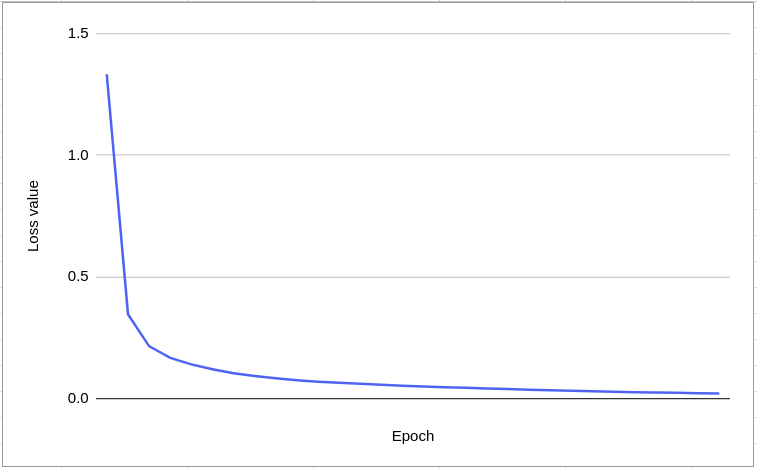
\includegraphics[width=1\linewidth]{training.png}
    \caption{Training loss per epoch}
    \label{fig:train_loss}
\end{figure}

The figure \ref{fig:train_loss} shows how the loss gradually decreases after each epoch. This shows that our model is learning as expected as the loss quickly drop in the first few epoch and slowly converge at the end.

Next, we could compare our model final result with some other existing baselines to make some final evaluation.
\begin{table}[H]
\centering
\begin{tabular}{|l|c|c|}
\hline
\textbf{Model} & \textbf{Accuracy (\%)} & \textbf{95\% Confidence Interval} \\
\hline
Logistic Regression & 94.8 & [93.8, 95.8] \\
Neural Network Classification & 96.3 & [95.3, 97.1] \\
Random Forest Classification & 96.8 & [96.1, 97.8] \\
Support Vector Classification & 97.5 & [96.5, 98.2] \\
XGBoost Classification & 96.1 & [95.1, 96.9] \\
\hline
\textbf{My CNN} & \textbf{96.0} & \textbf{-} \\
\hline
\end{tabular}
\vspace{0.2cm}
\caption{Performance Comparison of Classification Models}
\label{tab:model_comparison}
\end{table}


The final result actually shows that the model is only slightly better compared to Logistic Regression, comparable to Neural Network while performing slightly worse compared to others. At first sight, this could mean that our CNN is not performing well. However, notice that our data has a very small sized image. This means that there is relatively small number of features (only 64) and other models could still be able to capture patterns of the image. Additionally, we only build a relatively small model with only one convolution layer, so for the model to even be comparable with some other baselines could be considered as a promising result.

\section{Conclusion and Future works}
In conclusion, we have successfully build a Convolutional Neural Network and the result reveals its potential and ability to work on an image dataset comparing to some other baselines. However, the implementation is still lacking in the flexibility and the diversity of layers and architecture. It is clear that we can further extend the works by focusing on different activation or loss functions, extending Tensor class on many other operation like permute, or dot product, and finally to build some more complicated and advanced layer like skip connection, squeeze-and-excitation,... This will be the future works with more experiments on different tasks for CNNs.

\end{document}
